\chapter{Descripción del proyecto}

%\comA{Los aislantes topológicos pueden subclasificarse por la localización en la frontera de los estados en el gap. Las subclasificación se llama de orden superior y corresponde. Este trabajo esta inspirado en el trabajo publicado por Benalcazar at. all, en el articulo ''Quantized electric multipole insulators'' . La idea central es extender el modelo de SSH a un modelo 2-dimensional de forma cuadrada y otro en una forma de alfombra de Sierpinski, y así poder obtener HOTIs que tengan estados con densidades de probabilidad concentradas principalmente en las esquinas de la geometría. La tesis se enmarca en extender la aparición de hoti a redes fractales...
%}

Los aislantes topológicos están definidos por su relación bulto-frontera. Si un sistema de dimensión $d$ presenta estados con gap en el bulto y además presenta estados robustos ante perturbaciones sin gap en la frontera, se dice que este sistema es un aislante topológico. Sin embargo esta clasificación fue enriquecida con una subclasificación introducida por Benalcazar at. all \cite{Benalcazar2017} debido a sistemas que presentan estados sin gap en las aristas y los vértices, a esta subclasificación se le conoce como aislantes topológicos de orden superior (HOTI). Un aislante topológico de orden $n$-ésimo tiene estados protegidos sin gap en una frontera del sistema de codimensión $n$ \cite{schindler2018higher}.
Esta tesis se enfoca en extender la aparición de HOTI en redes fractales con dimensión de Housdorff fraccional, donde la relación de bulto y fronteras se desdibuja.  Esto se logró tomando el modelo utilizado por Benalcazar at. all en una red cuadrada y aplicarlo una red de Sierpinski.

    \section{Objetivo general}
    
    El objetivo de la tesis es extender la clasificación de aislantes topológicos de orden superior a redes de dimensión fractal, como lo es una red Sierpisnki cuadrada. También hacer un estudio que compare el comportamiento de las propiedades electrónicas de estados topológicos y no topológicos y su transición entre las redes cuadradas y redes de Sierpinski con los modelo Benalcazel, Bernevig, Taylor (BBT).

Particularmente, en los sistemas de geometría 2-dimensional se ha observados que al tener una transición adiabática de fase topológica a trivial y de trivial a topológica puede generar un bombeo de carga (Thouless pump \cite{benalcazar2020higher}) generado por el el flujo de los centros de Wannier. Debido a esto centramos nuestra atención en determinar si los HOTIs fractales también puede presentar bombeo de carga utilizando un modelos 2-dimensional inspirado en el modelo Rice-Mele.
    
    \section{Objetivo particular}
    \begin{itemize}
        \item Observar estados topológicos de orden superior en la red de Sierpinski y una red cristalina cuadrada.
        \item Caracterizar el cambio de la densidad (electrónica) de probabilidad en una transición de fase topológica a trivial. 
        \item Generar un espacio fase de la corriente como función de los parámetros $\gamma, \lambda$, con el fin de determinar cuándo el flujo de densidad de corriente será máximo.
        \item Determinar para que variación de parámetros existe bombeo de densidad de probabilidad en la red cristalina cuadrada y fractal.
    \end{itemize}
    
\section{Detalles de la implementación}
    

\subsection{Modelo BBH en una Red Cuadrada y en una alfombra de Sierpinski}\label{sec:Modelo_BBH_square_and_Fractal}

    Notemos que la idea del modelo de SSH se puede extender de manera sencilla, en algunos casos de 2 dimensiones, como lo es para una red cristalina cuadrada. Supongamos que tenemos una red cristalina cuadrada con 16 sitios y 4 redes unitarias (fig \ref{fig:Models} \textbf{(b)}) o celdas unitarias, cada una compuesta por 4 sitios como se ve en la (fig \ref{fig:Models} \textbf{(a)}), con $\gamma$ y $\lambda$ los parámetros de salto, intracelda e intercelda, respectivamente, con la particularidad de que cada que se pasa por la linea punteada el parametro de salta gana una fase de $-\pi$, por lo que nuestro sistema estaria compuesto, en las secciones horizontales, por cadenas de SSH en dirección positiva y dirección negativa intercaladas, y en la sección horizaontalen dir Siguiendo el modelo de SSH el hamitoniano de este sistema estará dado la matriz de conexión definida como la ecuación \ref{eq:BBH_Model_real} 
    
    
    \begin{figure}[h!]
     \centering
    \captionsetup[sub]{font=small}

     \begin{subfigure}[b!]{0.25 \textwidth}
         \caption{}
         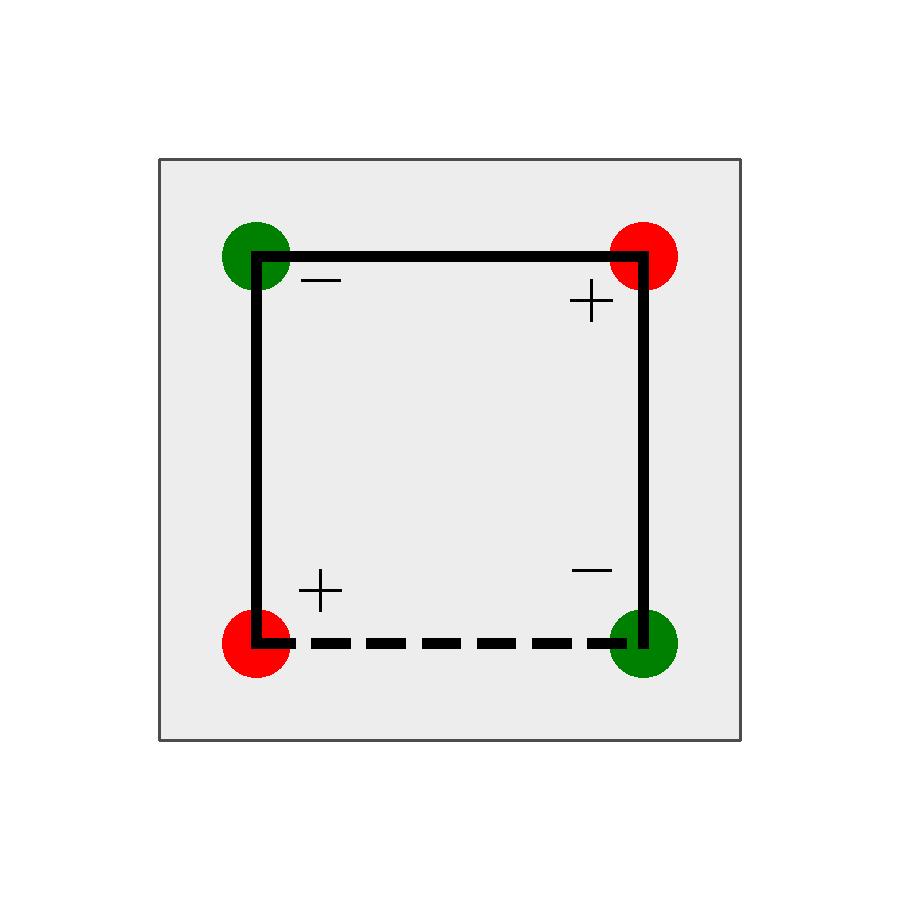
\includegraphics[width=\textwidth]{Imagenes/Models/unitary_cell.pdf}
     \end{subfigure}\hspace*{-0.5em}
     \begin{subfigure}[b!]{0.25 \textwidth}
         \caption{}
         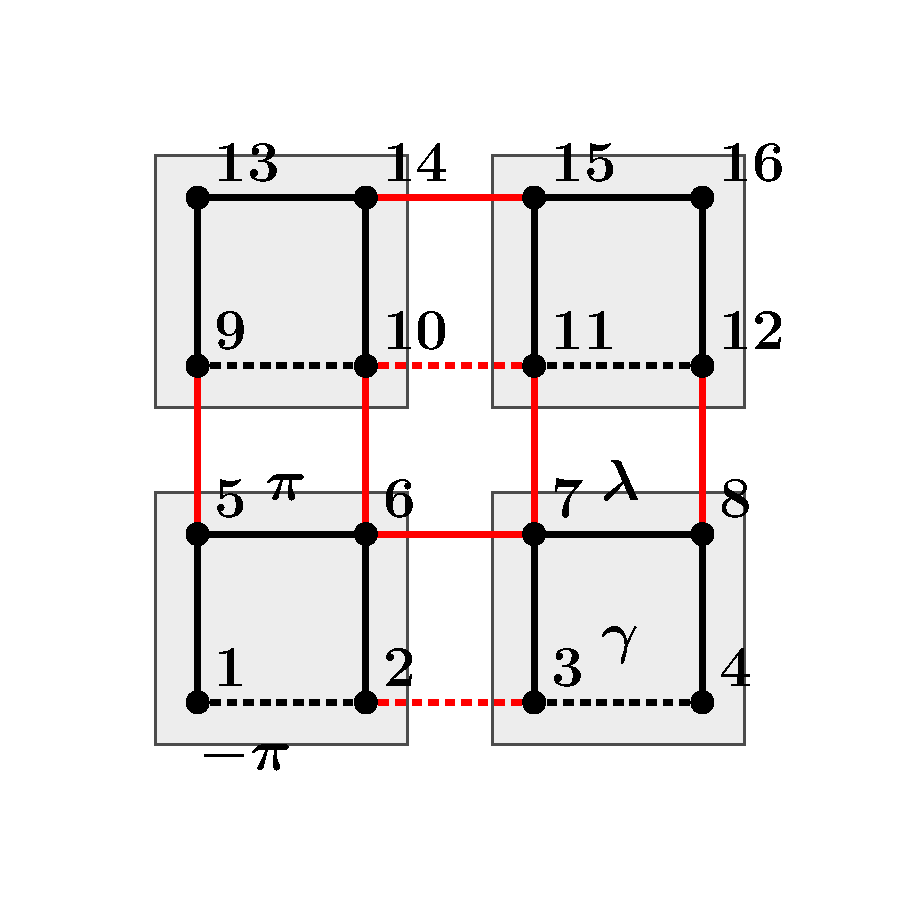
\includegraphics[width=\textwidth]{Imagenes/Models/square_hoti_model4.pdf}
     \end{subfigure}\hspace*{-0.3em}
     \begin{subfigure}[b!]{0.25 \textwidth}
         \caption{}
         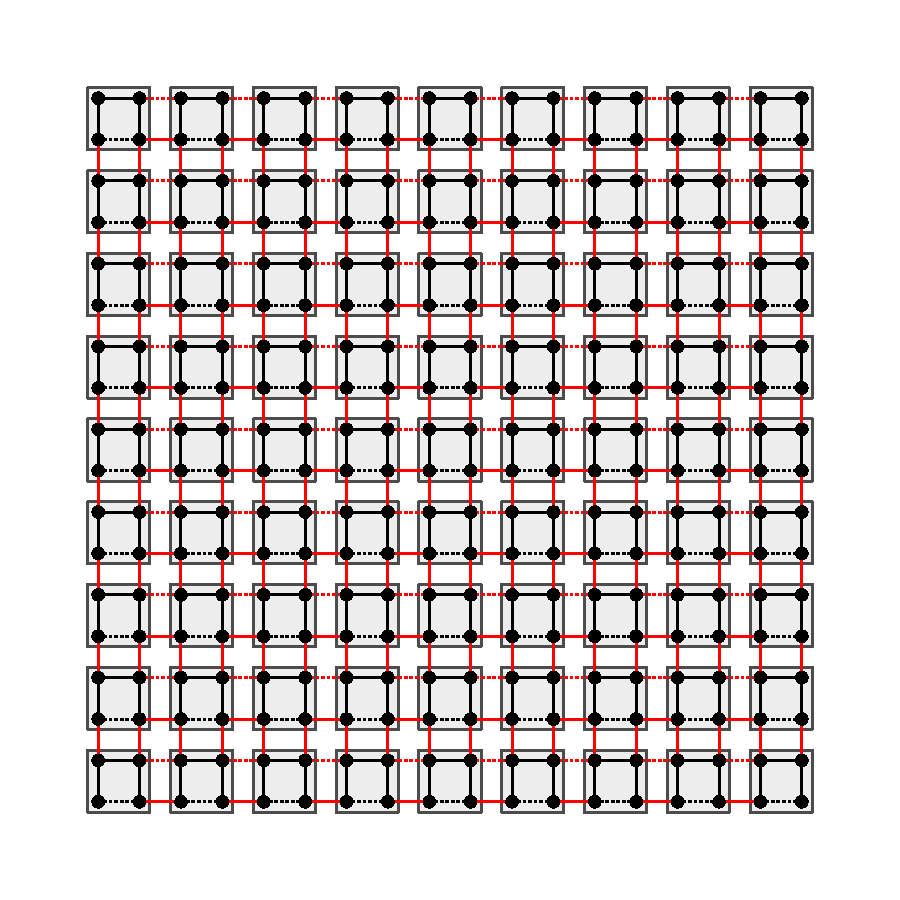
\includegraphics[width=\textwidth]{Imagenes/Models/square_hoti_model.pdf}
     \end{subfigure}\hspace*{-0.3em}
     \begin{subfigure}[b!]{0.25 \textwidth}
         \caption{}
         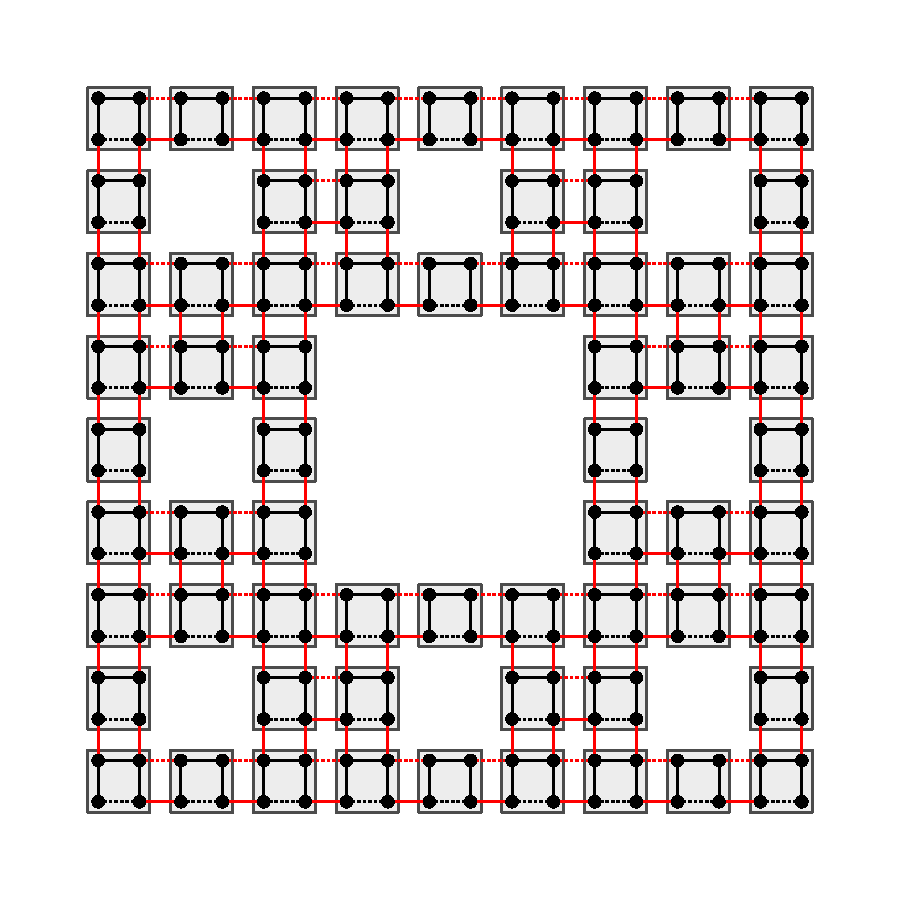
\includegraphics[width=\textwidth]{Imagenes/Models/fractal_hoti_model.pdf}
     \end{subfigure}
     
        \caption{\textbf{(a)} Celda unitaria de 4 sitios. \textbf{(b)} Red cristalina cuadrada de 4 celdas con 16 sitios. \textbf{(c)} Red cristalina cuadara conformada por 9x9 celdas y 18x18 sitios. \textbf{(d)} Red fractal conformada por 72 celdas y 288 sitios. }
        \label{fig:Models}
\end{figure}
    \label{eq:BBH_Model_real}
    \begin{equation} 
         H = 
     \begin{pmatrix}
        0 & -\gamma & 0 & 0 & \gamma & 0 & 0 & 0 & 0 & 0 & 0 & 0 & 0 & 0 & 0 & 0 & \\
        -\gamma & 0 & -\lambda & 0 &0 & \gamma & 0 & 0 & 0 & 0 & 0 & 0 & 0 & 0 & 0 & 0  \\
        0 & -\lambda & 0 & \gamma & 0 & 0 & \gamma & 0& 0 & 0 & 0 & 0 & 0 & 0 & 0 & 0 \\
        0 & 0 & -\gamma & 0 & 0 & 0 & 0 & \gamma  & 0 & 0 & 0 & 0 & 0 & 0 & 0 & 0 \\
        
        \gamma & 0 & 0 & 0 & 0 & \gamma & 0 & 0 & \lambda & 0 & 0 & 0 & 0 & 0 & 0 & 0 \\
        0 & \gamma & 0 & 0 & \gamma & 0 & \lambda & 0 & 0 & \lambda & 0 & 0 & 0 & 0 & 0 & 0 \\
        0 & 0 & \gamma & 0 & 0 & \lambda & 0 & \gamma & 0 & 0 & \lambda & 0 & 0 & 0 & 0 & 0 \\
        0 & 0 & 0 & \gamma & 0 & 0 & \gamma & 0 & 0 & 0 & 0 & \lambda & 0 &0 & 0 & 0 \\
        
        0 & 0 & 0 & 0 & \lambda & 0 & 0 & 0 & 0 & -\gamma & 0 & 0 & \gamma &0 & 0 & 0 \\
        0 & 0 & 0 & 0 & 0 & \lambda & 0 & 0 & -\gamma & 0 & -\lambda &  0 & 0 & \gamma & 0 & 0 \\
        0 & 0 & 0 & 0 & 0 & 0 & \lambda & 0 & 0 & -\lambda & 0 & -\gamma  &0 & 0 & \gamma & 0 \\
        0 & 0 & 0 & 0 & 0 & 0 & 0 & \lambda & 0 & 0 & -\gamma & 0 & 0 &0 & 0 & \gamma \\
        
        0 & 0 & 0 & 0 & 0 & 0 & 0 & 0 & \gamma & 0 & 0 & 0 & 0 & \gamma & 0 & 0 \\
        0 & 0 & 0 & 0 & 0 & 0 & 0 & 0 & 0 & \gamma & 0 & 0 & \gamma & 0 & \lambda & 0  \\
        0 & 0 & 0 & 0 & 0 & 0 & 0 & 0 & 0 & 0 & \gamma & 0 & 0 & \lambda & 0 & \gamma \\
        0 & 0 & 0 & 0 & 0 & 0 & 0 & 0 & 0 & 0 & 0 & \gamma & 0 & 0 & \gamma & 0 \\
        
    \end{pmatrix}
    \end{equation}
    
     
    Como podemos notar, las matrices que describen a estos sistemas son matrices de conexión por lo tanto es una matriz simétrica, de igual forma que en el caso uni-dimensional, es posible suponer condiciones periódicas a las frontera y obtener la matriz expresada en el espacio de momentos (eq.\ref{eq:BBH_Model_bloch}).
    
    \begin{equation}
    \label{eq:BBH_Model_bloch}
    H =      
     \begin{pmatrix}
            0 & -\gamma - \lambda e^{-ik_x} & \gamma + \lambda e^{-ik_y} &  0 \\
             -\gamma - \lambda e^{ik_x} & 0 &  0 & \gamma + \lambda e^{-ik_y}  \\
             \gamma + \lambda e^{ik_y} & 0 & 0 &  \gamma + \lambda e^{-ik_x} \\
             0 & \gamma + \lambda e^{ik_y} &  \gamma + \lambda e^{ik_x} & 0  \\
     \end{pmatrix} 
    \end{equation}

Donde $k_x$ y $k_y$ son las proyecciones del vector $\mathbf{k}$ de momentos sobre las direcciones $\mathbf{x}$ y $\mathbf{y}$, es decir, $\mathbf{k} = (k_x, k_y)$ este modelo se le conoce como modelo BBH (Benalcazar, Bernevig y Hughes). 


Ahora ¿Cómo implementamos la idea del HOTI cuadrado con el modelo de BBH en nuestra en una alfombra de Sierpinski? Una de las primeras cosas es notar como es el proceso iterativo de la construcción de una alfombra de Sierpinski, este proceso se describe la sección \ref{sc:Fractales}, para esta construcción se comenzó con un red crsitalina cuadrada inicial compuesta por 9 celdas unitarias y 36 sitos, a este cuadrado se le extrae la celda unitaria del centro, obteniendo una red como la de la figura \ref{fig:Fractals} \textbf{(b)}, esta idea sea itera $N=2$ veces obteniendo la red fractal que esperamos (fig. \ref{fig:Fractals} \textbf{(c)} y fig. \ref{fig:Models} \textbf{(d)} ), a diferencia del escalamiento que se observa en la construcción común de un fractal (fig. \ref{fig:Models}), para mantener las celdas con el mismo tamaño es necesario hacer el sistema cada vez mas grande. 

El hamitoniano que describe a este sistema estará dado por la matriz de conexión, sin embargo, dado que este sistema no tiene simetría traslación sobre la celda unitaria no es posible tener un hamiltoniano de Bloch que nos permita encontrar la solución en el espacio reciproco y así estudiar las propiedades electrónicas de las que nos podría proveer la teoría de bandas.

Debido a las limitantes computacionales el estudio de este sistema se fijo en la segunda  iteración ($N=2$) en la construcción del la alfombra de Sierpinski con 72 celdas y 288 sitios y el modelo de la red cuadrada se limito a un cuadrado compuesto por 81 celdas y 324 sitios. 

\subsection{Centros de Wannier en el espacio real}

Uno de los problemas principales al momento de calcular las cantidades topológicas como la fase de Berry en estructuras geométricas como los fractales es la falta de periodicidad en el sistema, lo cual no permite tener un hamiltoniano de Bloch que nos permita usar las expresiones \ref{eq:Barry_fase} para calcular la fase de Berry. Afortunadamente existen otras formas de construir este invariante sin necesidad de usar funciones de Bloch, y es a través del operador de posición, este nos permite extraer los centros de Wannier como eigenvalores de una cantidad llamada Wilson loop, esta forma es numéricamente estable y además es invariante de norma \cite{Asboth2015}.

Consideremos una cadena con $N$ elementos y largo $L$ con condiciones periódicas a la frontera, su operador de posición unitario estará dado por:
\begin{equation}
    \hat{X} = e^{i\delta_k \hat{x}}
\end{equation}
Con $\delta_k = L/N$. El valor esperado de la posición asociado al estado $\ket{\psi}$ se calculara como:
\begin{equation}
    \expectv{\hat{X}} = \frac{N}{2\pi} \; \text{arg} \; \sandwich{\psi}{\hat{X}}{\psi}
\end{equation}
Para poder calcular los centros de Wannier restringiremos el operador de posición únicamente a las bandas llenas:
\begin{equation}
    \hat{X}_P = \hat{P} \hat{X} \hat{P}
\end{equation}

Con $\hat{P} = \sum_{m = 1}^{N_{occ}} \sum_{k} \ket{\psi_{m,k}} \bra{\psi_{m,k}}$, para simplificar el operador $\hat{X}_P$  consideremos:
\begin{align}
    \sandwich{\psi_{m',k'}}{\hat{X}}{\psi_{m,k}} &= \frac{1}{N} \sum_{m'} e^{-im'k'} \bra{u_{m'}^{k'}}   \sum_{m} e^{im\delta_k} e^{imk}  \ket{u_{m}^{k}} \nonumber \\
    &=  \frac{1}{N} \braket{u_{m}^{k'}}{u_{m}^{k}} \sum_{m} e^{-im(k + \delta_k - k')} \nonumber \\
    &= \delta_{k + \delta_k, k'} \frac{1}{N} \braket{u_{m}^{k + \delta_k}}{u_{m}^{k}}  
\end{align}
Donde $\delta_{k + \delta_k, k'}$ sera $1$ cuando $k' = \delta_k + k$ y $0$ en cualquier otro caso, usando esto obtenemos:
\begin{align}
    \hat{X}_P &=  \sum_{m,m'=1}^{N_{occ}} \sum_{k,k'} \ket{\psi_{m',k'}} \bra{\psi_{m',k'}} \hat{X} \ket{\psi_{m,k}} \bra{\psi_{m,k}} \nonumber \\
    &= \sum_{m,n = 1}^{N_{occ}} \sum_{k} \ket{\psi_{n,k + \delta_k}} \braket{u_{n}^{k +\delta_k}}{u_{m}^{k}} \bra{\psi_{m,k}}
\end{align}
Podemos resolver la $N$-sima potencia de este sistema como un sistema de eigenvalores sobre el $m$-simo sitio ocupado:
\begin{equation}
    (\hat{X}_P)^N \ket{\nu^m} =  W \ket{\nu^m}
\end{equation}
Al termino de la derecha se le conoce como la linea de Wilson sobre un parametro ciclico, donde los elementos de matriz están conformados por las fases de Berry discretas sobre $k$:
\begin{equation}
    W_{i,j} = \delta_{i,j} \braket{u_m^{k+\delta_k}}{u_m^{k}} \braket{u_m^{k}}{u_m^{k-\delta_k}} \dots \braket{u_m^{k +2\pi -\delta_k}}{u_m^{k-2\pi}} 
\end{equation}
Donde $\delta_{i,j}$ es $1$ cuando $i = j+1$ y $0$ en otros casos. Con esto es posible determinar los centros de Wannier que estarán dados por los eigenvalores de la siguiente ecuacion ()

\begin{equation}
    W \ket{\nu^m}=(E^m)^N \ket{\nu^m}
\end{equation}

suponiendo que el Willson loop es un operador unitario, el problema se convierte en un problemas de fases ():
\begin{equation}
    (E^m)^N \ket{\nu^m} = e^{i2\pi\nu^m} \ket{\nu^m}
\end{equation}
Obteniendo como resultado final, la expresión de los centros de wanier asociados a la $m$-sima banda ocupada, en función del operador posición y el operador de proyección:

\begin{equation}
\label{eq:Wannier_center}
    \nu^m = \frac{N}{2\pi} \; \text{arg} \; \hat{X}_P
\end{equation}

 

%\comA{In the conventional Thouless pump [26, 33], an insulator with discrete translation symmetry adiabatically evolves in a periodic fashion leading to a quantization of the electron transport per cycle. The transport can be tracked by following the dipole moment in a crystal as the cycle progresses [34]. The change of the dipole moment over a cycle is a topologically-protected integer equal to the Chern number of the energy bands calculated in the 2D manifold spanned by the crystal momentum and the adiabatic parameter over that cycle [28].}